% ==============================================================================
% RECOMMENDED MAIN LATEX PREAMBLE SETUP FOR CLICKABLE BIBLIOGRAPHY:
% Copy these package configurations into your main thesis document (\main.tex)
% to enable fully clickable, clean hyperlinked citations, URLs, and DOIs:
%
% \usepackage[colorlinks=true, linkcolor=black, citecolor=blue, urlcolor=blue]{hyperref}
% \usepackage{doi} % Formats DOIs beautifully and makes them clickable
% ==============================================================================

\chapter{General Context and Project Framing}

\section{Introduction}
\textbf{Automation} and \textbf{Intent-Based Networking (IBN)} are driving modernization of the enterprise network infrastructure. In highly dynamic security environments, firewalls are an important enforcement point for security postures and require constant and accurate administration. The complexity of network management is due to the huge number of low-level device configurations, as shown in the seminal work by Benson et al. \cite{benson2009network}. In the past, network admins had to manually configure these devices, either through command-line interfaces (CLIs), graphical dashboards or static infrastructure-as-code (IaC) scripts. But at the scale of infrastructure and more dynamic operational needs, the cognitive load on administrators becomes much more significant. Configuration drift or delayed incident response from a cognitive burden is common; indeed, empirical analyses by Oppenheimer et al. \cite{oppenheimer2003why} suggest that \textbf{human configuration error} remains the primary driver of major internet service outages.

Embedding \textbf{conversational artificial intelligence} into infrastructure engineering is a potentially disruptive paradigm shift in the administration of systems. Advanced \textbf{Natural Language Understanding (NLU)} capabilities enable direct translation of abstract human intent to low-level configuration syntax. A recent evaluation by Wang et al. \cite{wang2024netconfeval} notes that Large Language Models (LLMs) can generate network commands effectively, but guarantees of their complete syntactic and semantic correctness remain a significant challenge. Enterprise networks need to be orchestrated with \textbf{deterministic behavior}, far from the \textbf{probabilistic vagueness} and \textbf{hallucination dangers} of probabilistic language models. Therefore, this project is based on the development of a secure hybrid AI-assisted network orchestration and FortiGate administration prototype. The system decouples conversational administration from a \textbf{strictly deterministic control plane}, closing the semantic gap between high-level intention and automated execution. In this chapter we present the background of the project, we discuss the main limitations of current paradigms and we introduce the architectural philosophy behind our prototype of secure orchestration.

\section{Host Organization Presentation}
This graduation project was conducted at the department of \textbf{cybersecurity and network engineering}, \textbf{Kleos}. We are experts in secure network architecture design, deployment and maintenance of enterprise networks. The research was motivated by the need to optimize administrative workflows, reduce mean time to resolution (MTTR) for operational requests, and simplify firewall management. We intend to be at the cutting edge of building a mature, \textbf{conversational operations assistant} with NLU capabilities without compromising the rigorous demands of secure systems engineering.

\section{Existing System Analysis}
The operational management of FortiGate appliances varies between \textbf{manual intervention} and \textbf{static automation}. Manual administration through FortiOS allows for nuanced decisions, but is inherently slow and prone to human error. In a detailed study of routing anomalies, Mahajan et al. \cite{mahajan2002understanding} demonstrated how small configuration errors can trigger cascading global effects. Static automation frameworks (e.g. Ansible or Terraform) on the other hand guarantee configuration consistency, but at the cost of considerable \textbf{operational rigidity}. Static policy-based systems such as CFEngine pioneered by Burgess \cite{burgess1995site} demand significant domain-specific expertise and are not designed to dynamically adapt to ad-hoc administrative queries or real-time conversational troubleshooting.

Recent attempts to introduce generic conversational agents into the network operations space have uncovered critical systemic gaps:
\begin{itemize}
    \item \textbf{No Active State Synchronization:} Generic assistants don’t have an active context of the current firewall configuration, so they propose changes that conflict with existing address objects or shadow existing routing rules. The lack of dynamic synchronization exacerbates this problem, often resulting in persistent deployment flaws, as demonstrated by empirical studies of configuration scripts by Rahman and Williams \cite{rahman2018characterizing}.
    \item \textbf{Lack of Entity Reconciliation:} Generic tools cannot deterministically reconcile ambiguous entities (e.g., ``the web server'') in unstructured network intents with live infrastructure objects.
    \item \textbf{Execution Imbalance:} The current paradigms often give the untrusted NLU interpreter direct execution capabilities, which contravenes fundamental infrastructure-as-code principles where execution must be predictable, verifiable and under strict control.
\end{itemize}

\section{Problem Statement}
The key challenge in modern network orchestration is not only executing commands but also understand intent correctly and reconciling with live operational environment safely. IBN requires a continuous closed loop that \textbf{translates, activates and verifies} intent against active system state according to Leivadeas and Falkner \cite{leivadeas2022survey}. While human error remains the main cause of security outages, critical infrastructure state transitions cannot be blindly trusted to fully automated, probabilistic systems. Recent work in software-defined networking emphasizes the importance of validating configurations before deployment to avoid severe connectivity loss.

The main problem studied in this thesis is: \textit{how to build a conversational administration prototype that reduces FortiGate operational workflows with AI-assisted natural language understanding, while adhering to strict \textbf{deterministic orchestration}, \textbf{active state synchronization} and \textbf{verifiable infrastructure-as-code} principles for configuration changes?}

\section{Project Objectives}
The main purpose of this thesis is to design architecturally mature hybrid network orchestration prototype. The particular engineering goals are:
\begin{enumerate} 
    \item \textbf{Conversational Administration:} Build a natural language interface to simplify complex FortiGate operations and reduce the cognitive burden for network operators.
    \item \textbf{Contextual Grounding \& Reconciliation:} Develop a strong entity extraction engine to map abstract human intents to exact FortiOS REST API schemas and live infrastructure objects.
    \item \textbf{Dynamic Routing Architecture:} Build a routing pipeline that separates read-only operational queries from state-mutating execution requests.
    \item \textbf{Deterministic Orchestration:} All API orchestration, validation and compliance checking must be done entirely in a deterministic Python control plane. This is consistent with the strict, automated testing paradigms proposed by Sokolowski et al. \cite{sokolowski2024automated} for verifying the safety of Infrastructure-as-Code programs before state changes are applied.
    \item \textbf{Infrastructure Lifecycle Management:} Add transaction-like state-restoration recovery protocols, employing active configuration snapshots and post-execution verification, to guarantee operational integrity and prevent partial state errors.
\end{enumerate}

\section{Proposed Solution: Deterministic AI-Assisted Orchestration}
We propose a solution in the form of a hybrid network orchestration prototype supported by NLU, specifically tailored to FortiGate environments. The system takes in natural language queries and routes them through a controlled routing pipeline. Routine operational queries and searches of documentation are passed through a \textbf{Retrieval-Augmented Generation (RAG)} architecture. RAG, as initially introduced by Lewis et al. \cite{lewis2020rag}, integrates pre-trained language models with dense vector retrieval to deliver precise, grounded, and contextually rich responses without the need for model retraining. RAG-enhanced architectures have been shown to be highly effective for parsing technical documentation and log files in network operations \cite{shajarian2024rag}. For administrative mutations, a dedicated NLU engine extracts structured intent that is immediately handed over to a deterministic Python orchestration backend. This control plane performs \textbf{entity reconciliation}, \textbf{forward-looking compliance checking}, \textbf{Human-in-the-Loop (HITL) approval} and \textbf{transactional API execution}. The platform is a hybrid AI-assisted operations assistant, streamlining the administrator’s workflow and enforcing strict security standards.

\section{Conceptual Architecture Philosophy}
The architectural philosophy of the platform is built upon the strict segregation of conversational interpretation and deterministic orchestration. In enterprise environments, the network state must be treated as \textbf{immutable} until systematically validated.

\begin{table}[H]
    \centering
    \caption{Division of Responsibilities: Probabilistic vs. Deterministic Planes}
    \label{tab:prob_vs_det}
    \renewcommand{\arraystretch}{1.5}
    \small
    \begin{tabular}{|p{3.5cm}|p{5.5cm}|p{5.5cm}|}
        \hline
        \textbf{Domain} & \textbf{Probabilistic Interpretation Plane (AI)} & \textbf{Deterministic Control Plane (Python)} \\
        \hline
        \textbf{Core Function} & Intent parsing, semantic understanding, unstructured data extraction. & API orchestration, state validation, execution, and verification. \\
        \hline
        \textbf{Data Handling} & Natural language to structured JSON mapping. & JSON schema validation, IP regex checks, entity reconciliation. \\
        \hline
        \textbf{Operational Context} & RAG-assisted contextual reference. & Live API state synchronization and lifecycle management. \\
        \hline
        \textbf{Execution Authority} & None. Strictly constrained to interpretation. & Absolute authority over all API state mutations. \\
        \hline
    \end{tabular}
\end{table}

By formalizing this division, the architecture ensures that the AI is utilized exclusively for its strengths in semantic mapping, while the Python backend guarantees the \textbf{idempotency, safety, and predictability} required in professional network engineering.

\section{Logical System Architecture \& Trust Boundaries}
The global architecture is designed to orchestrate the complete lifecycle of an administrative request from conversational ingestion to final verification.

\begin{figure}[H]
    \centering
    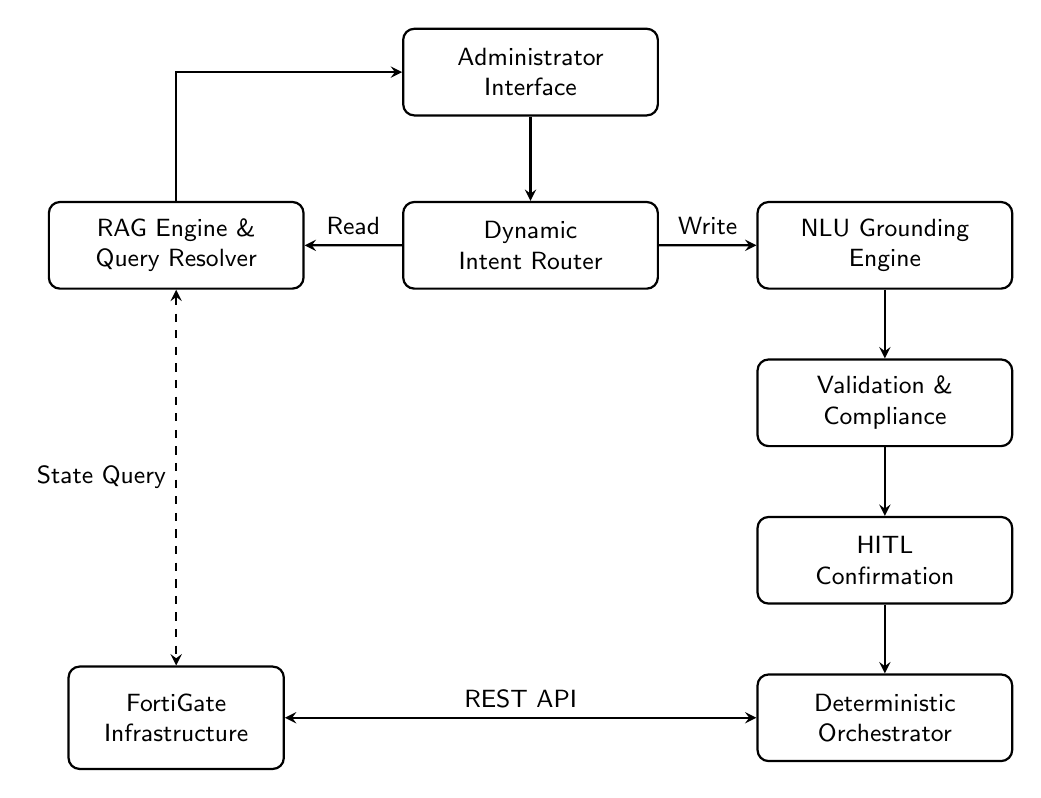
\begin{tikzpicture}[
        node distance=2.2cm,
        every node/.style={font=\sffamily\small},
        component/.style={rectangle, draw=black, thick, fill=white, text width=3.0cm, align=center, minimum height=1.1cm, rounded corners},
        database/.style={rectangle, draw=black, thick, fill=white, text width=2.5cm, align=center, minimum height=1.3cm, rounded corners},
        arrow/.style={->, thick, draw=black, >=stealth}
        ]
        
        % Symmetrical Layout Nodes
        \node[component, fill=white] (user) at (0, 0) {Administrator\\Interface};
        \node[component, below of=user, node distance=2.2cm] (router) {Dynamic\\Intent Router};
        
        % Left Side: Read-Only Path
        \node[component] (rag) at (-4.5, -2.2) {RAG Engine \&\\Query Resolver};
        \node[database] (fortigate) at (-4.5, -8.2) {FortiGate\\Infrastructure};
        
        % Right Side: Write Mutation Path
        \node[component] (grounding) at (4.5, -2.2) {NLU Grounding\\Engine};
        \node[component] (validator) at (4.5, -4.2) {Validation \&\\Compliance};
        \node[component] (hitl) at (4.5, -6.2) {HITL\\Confirmation};
        \node[component] (executor) at (4.5, -8.2) {Deterministic\\Orchestrator};
        
        % Orderly Connections (No Crossings)
        \draw[arrow] (user) -- (router);
        \draw[arrow] (router) -- node[above] {Read} (rag);
        \draw[arrow] (router) -- node[above] {Write} (grounding);
        \draw[arrow] (rag) |- (user);
        \draw[arrow] (grounding) -- (validator);
        \draw[arrow] (validator) -- (hitl);
        \draw[arrow] (hitl) -- (executor);
        \draw[arrow, <->] (executor) -- node[above] {REST API} (fortigate);
        \draw[arrow, <->, dashed] (rag) -- node[left] {State Query} (fortigate);
        
    \end{tikzpicture}
    \caption{Global Platform Architecture and Component Interaction}
    \label{fig:global_arch}
\end{figure}

One important part of this design is to establish hard \textbf{trust boundaries}. All outputs of probabilistic language models are treated as \textbf{unvalidated data} by the system until they pass the \textbf{deterministic validation threshold}. This is in line with the interactive machine learning paradigm explored by Gómez-Carmona et al. \cite{gomez2024hitl}, which aims to keep the human in the loop to review and validate complex decisions, so that automated systems can be kept safe, interpretable, and under tight human supervision.

\begin{figure}[H]
    \centering
    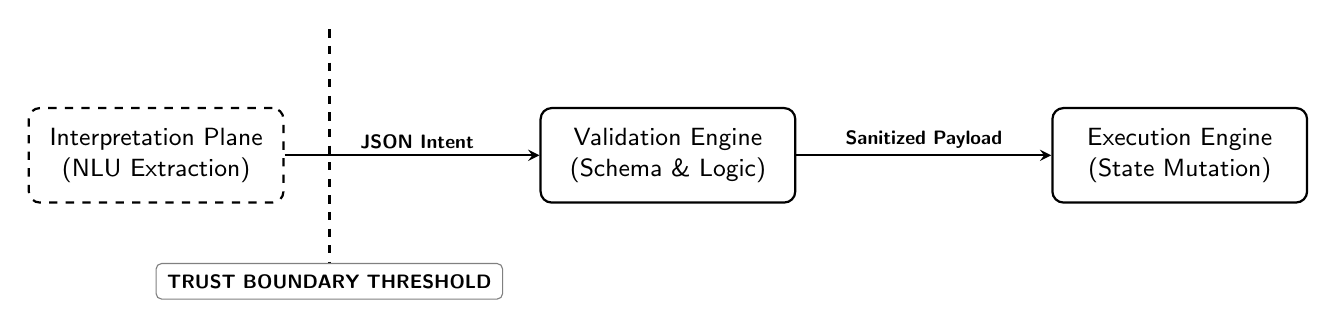
\begin{tikzpicture}[
        node distance=2.5cm,
        every node/.style={font=\sffamily\small},
        untrusted/.style={rectangle, draw=black, thick, dashed, fill=white, text width=3.0cm, align=center, minimum height=1.2cm, rounded corners},
        trusted/.style={rectangle, draw=black, thick, fill=white, text width=3.0cm, align=center, minimum height=1.2cm, rounded corners},
        arrow/.style={->, thick, draw=black, >=stealth},
        badge/.style={fill=white, font=\sffamily\scriptsize\bfseries, inner sep=2pt}
        ]
        
        % Symmetrical and Widened Node Placements (6.5cm center-to-center distance)
        \node[untrusted] (llm) at (0, 0) {Interpretation Plane\\(NLU Extraction)};
        \node[trusted] (val) at (6.5, 0) {Validation Engine\\(Schema \& Logic)};
        \node[trusted] (exec) at (13.0, 0) {Execution Engine\\(State Mutation)};
        
        % Vertical Boundary Line perfectly positioned at x = 2.2
        \draw[black, very thick, dashed] (2.2, 1.6) -- (2.2, -1.6);
        
        % Clean Monochrome Boundary Label at the Bottom, aligned at x = 2.2
        \node[draw=black!50, fill=white, rounded corners=2pt, font=\sffamily\scriptsize\bfseries, inner sep=4pt] at (2.2, -1.6) {TRUST BOUNDARY THRESHOLD};
        
        % Connections with perfect middle-right positioning (Zero overlapping)
        \draw[arrow] (llm) -- node[above, pos=0.52, badge] {JSON Intent} (val);
        \draw[arrow] (val) -- node[above, pos=0.5, badge] {Sanitized Payload} (exec);
        
    \end{tikzpicture}
    \caption{Trust Boundary Architecture separating Interpretation and Control Planes}
    \label{fig:trust_boundary}
\end{figure}

\section{Conceptual Routing \& Intent Flow}
The platform is designed with a dynamic intent routing architecture that enables interaction with infrastructure and guarantees the safety of operations. The router does not give equal treatment to all conversational inputs, but classifies the intent to enforce structural \textbf{Read/Write operational isolation}.

\begin{table}[H]
    \centering
    \caption{Intent Classification and Routing Architecture}
    \label{tab:routing_class}
    \renewcommand{\arraystretch}{1.5}
    \small
    \begin{tabular}{|l|p{5cm}|p{6.5cm}|}
        \hline
        \textbf{Operation Class} & \textbf{Routing Destination} & \textbf{Architectural Objective} \\
        \hline
        \textbf{State Query} & Live API Read Engine & Retrieve current interface status, active policies, or system health directly from the infrastructure. \\
        \hline
        \textbf{Knowledge Query} & RAG Reference Engine & Query indexed Fortinet documentation to assist the administrator. \\
        \hline
        \textbf{Mutation Request} & NLU Grounding Pipeline & Extract structured intent for creating, modifying, or deleting operational configurations. \\
        \hline
        \textbf{Ambiguous Intent} & Clarification Loop & Reject vague requests and logically prompt the user for mandatory operational parameters. \\
        \hline
    \end{tabular}
\end{table}

\section{High-Level Grounding Concepts}
A primary engineering issue encountered in intent-based orchestration systems is converting vague human references into strict infrastructure identifiers. This semantic conversion process is accomplished by the \textbf{Grounding Engine}. For instance, if an administrator requests to "block traffic from the web servers," then the NLU will extract the entity concept. Following this extraction, the deterministic \textbf{reconciliation engine} queries the live FortiGate state to obtain the exact address object names or IP subnets needed by the underlying API corresponding to "web servers."

If an entity cannot be definitively resolved against the live infrastructure state, or if required operational parameters are missing, the system initiates a \textbf{Conversational Clarification Loop}. This workflow ensures the platform behaves as a collaborative administrative assistant, persistently requesting specific context until the intent is deterministically sound.

\section{Operational Processing Pipeline}
To ensure deterministic execution, every mutation request traverses a rigorous operational lifecycle. This pipeline acts as a sequential state machine, guiding an administrative request from its initial natural language ingestion, through entity grounding and human-in-the-loop review, down to the final REST API orchestration and verification. The deeply technical execution mechanics of this lifecycle, including the multi-phase transition matrix, are explored extensively in Chapter 3.

\section{Validation \& Compliance Strategy}
Before any configuration payload reaches the execution layer, it is subjected to a multi-tiered validation strategy. This strategy enforces structural integrity (syntactic checking), dynamic reconciliation (semantic grounding), and strict organizational security postures (proactive compliance). By validating intents conceptually before they are executed physically, the platform prevents misconfigurations. The mathematical logic driving these compliance gates is detailed in the architectural design sections of Chapter 3.

\section{Infrastructure Lifecycle Management}
While conversational interpretation forms the probabilistic layer of the platform, robust infrastructure-as-code principles mandate fail-safe execution mechanics. Network configurations are intrinsically stateful; partial API updates can inadvertently sever remote administrative access. Consequently, the platform embeds snapshot and state-restoration (rollback) protocols natively into the orchestration engine. This guarantees transaction-like safety for all administrative modifications, the programmatic implementation of which is analyzed in Chapter 3.

\section{Methodology and Task Distribution}
The project was executed utilizing an \textbf{Agile engineering methodology}, incorporating iterative sprints to progressively build, integrate, and harden the architecture. This approach facilitated the continuous refinement of the conversational interface while rigorously testing the deterministic API orchestration against simulated enterprise topologies.

\begin{table}[H]
    \centering
    \caption{Agile Development Phases and Project Milestones}
    \label{tab:project_phases}
    \renewcommand{\arraystretch}{1.5}
    \small
    \begin{tabular}{|p{3.5cm}|p{9cm}|}
        \hline
        \textbf{Engineering Phase} & \textbf{Core Deliverables and Focus Areas} \\
        \hline
        \textbf{Architecture Design} & State of the art analysis, system modeling, defining trust boundaries, and read/write separation models. \\
        \hline
        \textbf{API Orchestration} & Development of the deterministic Python backend, state synchronization, snapshot, and restoration modules. \\
        \hline
        \textbf{Intelligence Layer} & Implementation of the NLU grounding pipeline, entity reconciliation, and the intent routing architecture. \\
        \hline
        \textbf{Workflow Refinement} & Integration of the clarification loop, HITL interfaces, and proactive compliance enforcement. \\
        \hline
        \textbf{Validation} & Comprehensive system testing, latency optimization, and verification against complex edge-case network scenarios. \\
        \hline
    \end{tabular}
\end{table}

\section{Project Planning}
The implementation and orchestration of this graduation project were arranged in a sequential manner to address the critical dependencies between the deterministic execution layers and probabilistic conversational interfaces. A first engineering phase focused on developing and hardening the deterministic Python orchestration engine, with all API bindings, state recovery snapshots and verification pipelines thoroughly tested. NLU grounding layer and RAG capabilities were then combined and deployed Human-in-the-Loop (HITL) workflow and conversational clarification loops.

The project was divided into five discrete phases in order with a total of 12 weeks (3 months) duration for professional engineering and strict schedule follow-up. Figure~\ref{fig:project_roadmap} shows the roadmap of the visual execution. The vertical waterfall of engineering sprints and the dashed trigger points for core project milestones.

\begin{figure}[H]
    \centering
    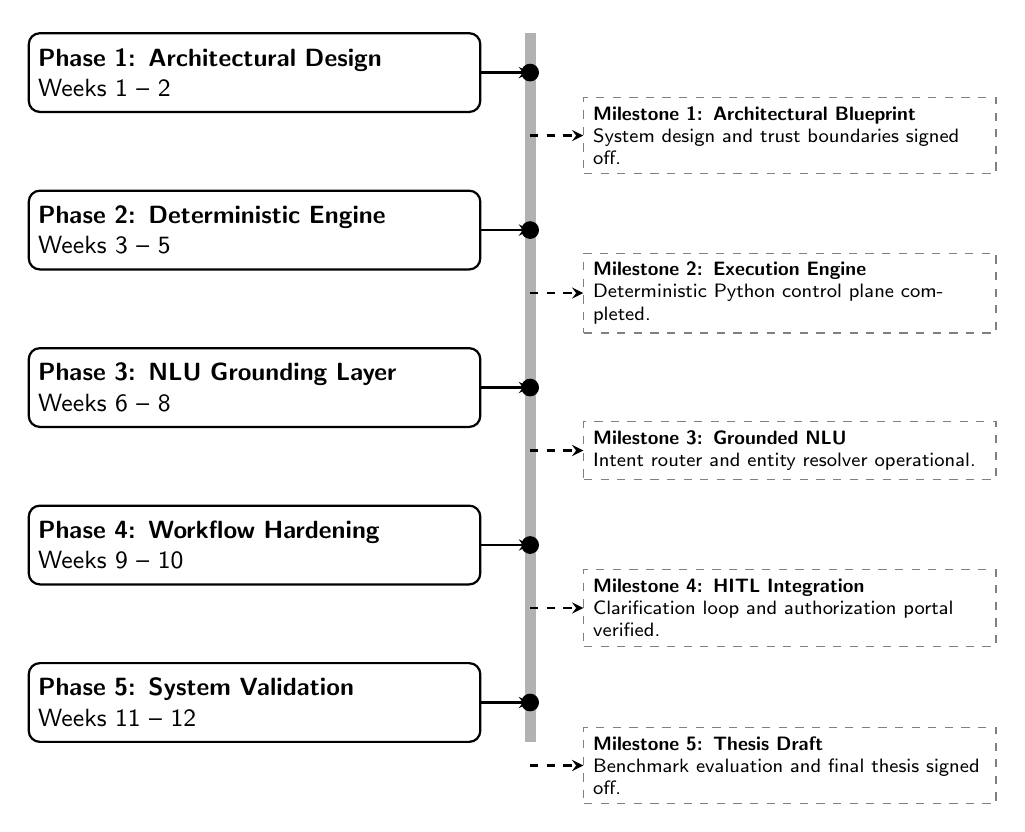
\begin{tikzpicture}[
        node distance=1.5cm,
        every node/.style={font=\sffamily\small},
        phase/.style={rectangle, draw=black, thick, fill=white, text width=5.5cm, align=left, minimum height=1.0cm, rounded corners},
        milestone/.style={rectangle, draw=black!50, dashed, fill=white, text width=5.0cm, align=left, font=\sffamily\scriptsize},
        arrow/.style={->, thick, draw=black, >=stealth}
        ]
        
        % Vertical timeline track
        \draw[black!30, line width=4pt] (0, 0.5) -- (0, -8.5);
        
        % Phase Nodes (Left of track)
        \node[phase] (p1) at (-3.5, 0) {\textbf{Phase 1: Architectural Design}\\Weeks 1 -- 2};
        \node[phase] (p2) at (-3.5, -2.0) {\textbf{Phase 2: Deterministic Engine}\\Weeks 3 -- 5};
        \node[phase] (p3) at (-3.5, -4.0) {\textbf{Phase 3: NLU Grounding Layer}\\Weeks 6 -- 8};
        \node[phase] (p4) at (-3.5, -6.0) {\textbf{Phase 4: Workflow Hardening}\\Weeks 9 -- 10};
        \node[phase] (p5) at (-3.5, -8.0) {\textbf{Phase 5: System Validation}\\Weeks 11 -- 12};
        
        % Milestone Nodes (Right of track)
        \node[milestone] (m1) at (3.3, -0.8) {\textbf{Milestone 1: Architectural Blueprint}\\System design and trust boundaries signed off.};
        \node[milestone] (m2) at (3.3, -2.8) {\textbf{Milestone 2: Execution Engine}\\Deterministic Python control plane completed.};
        \node[milestone] (m3) at (3.3, -4.8) {\textbf{Milestone 3: Grounded NLU}\\Intent router and entity resolver operational.};
        \node[milestone] (m4) at (3.3, -6.8) {\textbf{Milestone 4: HITL Integration}\\Clarification loop and authorization portal verified.};
        \node[milestone] (m5) at (3.3, -8.8) {\textbf{Milestone 5: Thesis Draft}\\Benchmark evaluation and final thesis signed off.};
        
        % Horizontal marker circles on track
        \filldraw[black] (0, 0) circle (3pt);
        \filldraw[black] (0, -2.0) circle (3pt);
        \filldraw[black] (0, -4.0) circle (3pt);
        \filldraw[black] (0, -6.0) circle (3pt);
        \filldraw[black] (0, -8.0) circle (3pt);
        
        % Connection lines
        \draw[arrow] (p1.east) -- (0, 0);
        \draw[arrow] (p2.east) -- (0, -2.0);
        \draw[arrow] (p3.east) -- (0, -4.0);
        \draw[arrow] (p4.east) -- (0, -6.0);
        \draw[arrow] (p5.east) -- (0, -8.0);
        
        \draw[arrow, dashed] (0, -0.8) -- (m1.west);
        \draw[arrow, dashed] (0, -2.8) -- (m2.west);
        \draw[arrow, dashed] (0, -4.8) -- (m3.west);
        \draw[arrow, dashed] (0, -6.8) -- (m4.west);
        \draw[arrow, dashed] (0, -8.8) -- (m5.west);
        
    \end{tikzpicture}
    \caption{Project Planning Roadmap: Sprints and Milestone Execution}
    \label{fig:project_roadmap}
\end{figure}

Complementing the visual roadmap, Table~\ref{tab:sprint_planning} outlines the detailed schedule of development sprints, core engineering tasks, and concrete academic deliverables for each phase of the project lifecycle.

\begin{table}[H]
    \centering
    \caption{Project Planning: Sprint Timeline, Tasks, and Key Deliverables}
    \label{tab:sprint_planning}
    \renewcommand{\arraystretch}{1.4}
    \small
    \begin{tabular}{|l|c|p{4.8cm}|p{5.2cm}|}
        \hline
        \textbf{Project Phase} & \textbf{Timeline} & \textbf{Core Tasks \& Sprints} & \textbf{Key Deliverables} \\
        \hline
        \textbf{Phase 1: Architecture} & Weeks 1--2 & Literature review, state-of-the-art analysis, architectural system design. & Sign-off on system architecture and trust boundary definitions. \\
        \hline
        \textbf{Phase 2: Execution} & Weeks 3--5 & Development of deterministic Python REST API wrappers, local state snapshot mechanisms, validation modules. & Fully functional API orchestration control plane with rollback capabilities. \\
        \hline
        \textbf{Phase 3: NLU Layer} & Weeks 6--8 & Intent router training, entity extraction models, RAG vector database indexing for technical documentation. & Trained intent router and operational RAG-assisted knowledge query resolver. \\
        \hline
        \textbf{Phase 4: Workflow} & Weeks 9--10 & Human-in-the-Loop web portal integration, conversation clarification loops, policy verification hooks. & Dual-interface (Streamlit admin panel and HITL approval portal) fully coupled with backend. \\
        \hline
        \textbf{Phase 5: Validation} & Weeks 11--12 & Synthetic load testing, latency benchmarking, configuration error recovery checks, final report writing. & Complete benchmark analysis, performance evaluation metrics, and thesis submission. \\
        \hline
    \end{tabular}
\end{table}

\section{Report Organization}
The remainder of this thesis is structured as follows:
\begin{itemize}
    \item \textbf{Chapter 2: State of the Art and Theoretical Background:} Explores modern infrastructure automation, the evolution of Intent-Based Networking (IBN), and the integration of conversational interfaces in systems engineering.
    \item \textbf{Chapter 3: System Design and Architecture:} Details the conceptual, structural, and detailed design of the system, including the routing engine, entity grounding, validation compliance algorithms, and UML diagrams.
    \item \textbf{Chapter 4: Implementation, Testing, and Validation:} Showcases the implementation environment, the Streamlit user interface, experimental test cases (grounding, compliance blocks, and rollbacks), performance results, and system limitations.
\end{itemize}

\section{Chapter Conclusion}
The introduction to the subject matter and engineering scope of the project is the purpose of this chapter. As we assessed the complexity of today's infrastructure management, we discovered an \textbf{operational gap} (i.e., not to be confused with gaps related to processes) where the degree of flexibility of conversational AI does not meet the degree of dependability required for professional orchestration in this context. Through a well-developed \textbf{hybrid architectural solution}, this platform addresses the gap between the operational flexibility of conversational artificial intelligence (AI) and the absolute dependability of professional orchestration (a case study in the previous section of the introduction section of this document) by creating a secure operational assistant that leverages technology to provide \textbf{controlled routing}, \textbf{accurate object grounding} (which the next chapter covers), \textbf{live state reconciliation}, and \textbf{deterministic validation}.

The \textbf{rigorous lifecycle management processes} incorporated into the platform (i.e., \textbf{compliance}, \textbf{Human-in-the-Loop (HITL) authorization}, and \textbf{validation}) lend themselves to improving the use of natural language to manage enterprise security architectures while protecting the integrity of these systems in a deterministic manner. The following chapters will provide a more in-depth look at the theoretical approaches and implementation technologies that will enable the next generation of orchestration platforms to be operationalized.
